\documentclass{beamer}

\usetheme{Madrid}   % Clean and common
\usepackage{graphicx}
\usepackage{tikz}
\usetikzlibrary{decorations.pathreplacing}
\usepackage{listings}
\usepackage{amsmath}
\usepackage{amssymb}

\title{Knuth-Morris-Pratt (KMP) String Matching}
\subtitle{CSE 200:Technical Writing and Presentation}
\author[Group 1]{%
  Ragib Al-Hasib - 2305152\\
  Saleh Mustabir Rafi - 2305153\\
  Abdus Sakur Sifat - 2305154}

\date{\today}

\begin{document}


% =====================================================================
%  PART 2 -- continues the frame count from Part 1 (Introduction ...
%  LPS Construction Simulation). Only the frames below are new; the
%  preamble/title are repeated here only so this file compiles on its
%  own. When merging insadasto the master deck, copy just the
%  \begin{frame} ... \end{frame} blocks below (skip the duplicate
%  preamble and titlepage), and make sure \usepackage{amssymb} is
%  added once to the shared preamble (needed for \checkmark).
% =====================================================================

\begin{frame}{From Preprocessing to Searching}
\noindent{\Large\bfseries Where We Left Off\par}
\vspace{0.4cm}

\onslide<1->{%
\begin{itemize}
  \item The \textbf{LPS array} is built once, in $O(m)$ time
  \item It tells us: \emph{if a mismatch happens here, how far can we safely skip?}
\end{itemize}
}

\vspace{0.6cm}

\onslide<2->{%
\noindent{\large\bfseries Now: Put LPS to Work\par}
\begin{itemize}
  \item Scan the text just \textbf{once}, left to right
  \item Use LPS to \textbf{avoid re-checking} characters we already know match
  \item Goal: find every occurrence of the pattern in $O(n+m)$ time
\end{itemize}
}
\end{frame}

\begin{frame}{Two Pointers: The Core Idea}
\noindent{\Large\bfseries Meet $i$ and $j$\par}
\vspace{0.3cm}

\onslide<1->{%
\begin{itemize}
  \item $i$ walks along the \textbf{text}, from $0$ to $n$
  \item $j$ walks along the \textbf{pattern}, from $0$ to $m$
  \item Characters \textbf{match} $\Rightarrow$ advance \textit{both} $i$ and $j$
  \item Characters \textbf{mismatch} $\Rightarrow$ move \textit{only} $j$, guided by LPS
\end{itemize}
}

\vspace{0.7cm}

\onslide<2->{%
\begin{alertblock}{The Golden Rule}
\centering\Large $i$ never moves backward.
\end{alertblock}
}

\vspace{0.4cm}
\onslide<3->{%
\begin{center}
\footnotesize This is exactly what the naive approach could \textbf{not} do --- it restarts $i$ from scratch at every new position.
\end{center}
}
\end{frame}

\begin{frame}{The Aha Moment: Reusing Overlaps}
\noindent{\large\bfseries Recall: $S=$\texttt{ABAB}, \ $LPS=[0,0,1,2]$\par}
\vspace{0.1cm}
\centering
\begin{tikzpicture}[x=0.85cm,y=1cm]
\path[use as bounding box] (-1.6,-1.7) rectangle (7.3,3.1);

\node[anchor=east] at (-0.4,0.35) {Text:};
\foreach \letter [count=\p from 0] in {A,B,A,B,A,B} {
  \draw (\p,0) rectangle (\p+1,0.7);
  \node[font=\ttfamily\large] at (\p+0.5,0.35) {\letter};
  \node[font=\scriptsize] at (\p+0.5,-0.3) {\p};
}
\node[anchor=east] at (-0.4,2.0) {Pattern:};

\only<1>{
  \foreach \p in {0,1,2,3} {
    \fill[green!22] (\p,1.65) rectangle (\p+1,2.35);
    \draw (\p,1.65) rectangle (\p+1,2.35);
  }
  \foreach \letter [count=\p from 0] in {A,B,A,B} {
    \node[font=\ttfamily\large] at (\p+0.5,2.0) {\letter};
  }
  \draw[green!40!black,very thick] (0,1.65) rectangle (4,2.35);
  \draw[green!40!black,very thick] (0,0) rectangle (4,0.7);
  \node[anchor=north,align=center,text width=6.8cm,font=\small] at (3.5,-0.65)
    {\textcolor{green!40!black}{\checkmark} Full match at index \textbf{0}! Since $LPS[3]=2$, jump straight to $j=2$ --- keep \texttt{AB}, no need to recheck it.};
}

\only<2>{
  \foreach \p in {2,3} {
    \fill[yellow!20] (\p,1.65) rectangle (\p+1,2.35);
    \draw[black!40] (\p,1.65) rectangle (\p+1,2.35);
  }
  \foreach \p in {4,5} {
    \fill[green!22] (\p,1.65) rectangle (\p+1,2.35);
    \draw (\p,1.65) rectangle (\p+1,2.35);
  }
  \foreach \letter [count=\i from 0] in {A,B,A,B} {
    \node[font=\ttfamily\large] at (2+\i+0.5,2.0) {\letter};
  }
  \draw[green!40!black,very thick] (2,1.65) rectangle (6,2.35);
  \draw[green!40!black,very thick] (2,0) rectangle (6,0.7);
  \node[anchor=north,align=center,text width=6.8cm,font=\small] at (3.5,-0.65)
    {\textcolor{green!40!black}{\checkmark} Full match at index \textbf{2}! Two overlapping matches, found with \textbf{zero} wasted comparisons and \textbf{no} backward move of $i$.};
}
\end{tikzpicture}
\end{frame}

\begin{frame}{KMP Search Algorithm}
\noindent{\Large\bfseries Scanning the Text\par}
\vspace{0.4cm}

\onslide<1->{%
\begin{tabular}{@{}r c l@{}}
$i$ & = & current position in the \textbf{text} \\[3pt]
$j$ & = & current position in the \textbf{pattern} \\[3pt]
$n,\ m$ & = & lengths of the text and pattern
\end{tabular}
}

\vspace{0.7cm}

\onslide<2->{%
\small
\[
\text{Step}(i,j) \;=\; \left\{
\begin{array}{ll}
(i+1,\ j+1) & \text{if } T[i]=P[j] \quad\text{\scriptsize(match --- advance both)}\\[6pt]
(i,\ LPS[j-1]) & \text{if } T[i]\neq P[j],\ j>0 \quad\text{\scriptsize(fall back, keep $i$)}\\[6pt]
(i+1,\ 0) & \text{if } T[i]\neq P[j],\ j=0 \quad\text{\scriptsize(advance $i$ only)}
\end{array}
\right.
\]
}

\vspace{0.4cm}
\onslide<3->{%
\begin{center}
\large Whenever $j$ reaches $m$: \textbf{report a match} at index $i-m$, then set $j \leftarrow LPS[m-1]$.
\end{center}
}
\end{frame}

\begin{frame}{KMP Search: Pseudocode}
\noindent{\Large\bfseries Putting It Into Code\par}
\vspace{0.15cm}

\onslide<1->{%
\begin{exampleblock}{KMP-Search$(T,\,P,\,LPS)$}
\ttfamily\footnotesize
$n \leftarrow$ length$(T)$\qquad $m \leftarrow$ length$(P)$\\
$i \leftarrow 0$\qquad $j \leftarrow 0$\\[3pt]
\textbf{while} $i < n$:\\
\quad\textbf{if} $T[i] = P[j]$:\\
\quad\quad $i \leftarrow i+1$\qquad $j \leftarrow j+1$\\
\quad\quad \textbf{if} $j = m$:\\
\quad\quad\quad \textbf{report} match at index $i-m$\\
\quad\quad\quad $j \leftarrow LPS[j-1]$\\
\quad\textbf{else if} $j > 0$:\\
\quad\quad $j \leftarrow LPS[j-1]$\\
\quad\textbf{else}:\\
\quad\quad $i \leftarrow i+1$
\end{exampleblock}
}

\vspace{0.2cm}
\onslide<2->{%
\begin{center}
\footnotesize Exactly the same three rules from the previous slide --- now written as code we could actually run.
\end{center}
}
\end{frame}

\begin{frame}{KMP Search Simulation}
\noindent{\small\bfseries Warm-up example: $T=$\texttt{aabaacaadaabaaba},\ $P=$\texttt{aaba},\ $LPS=[0,1,0,1]$\par}
\vspace{-0.05cm}
\centering
\begin{tikzpicture}[x=0.58cm,y=0.85cm]
\path[use as bounding box] (-2.4,-2.3) rectangle (16.6,3.1);

\only<1-13>{
\node[anchor=west,font=\scriptsize] at (-2.3,2.6)
  {\colorbox{yellow!20}{\phantom{x}}\,inherited \quad
   \colorbox{green!22}{\phantom{x}}\,match \quad
   \colorbox{red!18}{\phantom{x}}\,mismatch};
}

\node[anchor=east] at (-0.3,0.3) {Text:};
\foreach \letter [count=\p from 0] in {a,a,b,a,a,c,a,a,d,a,a,b,a,a,b,a} {
  \draw (\p,0) rectangle (\p+1,0.6);
  \node[font=\ttfamily\large] at (\p+0.5,0.3) {\letter};
  \node[font=\scriptsize] at (\p+0.5,-0.28) {\p};
}
\only<1-13>{\node[anchor=east] at (-0.3,1.5) {Pattern:};}

\only<1->{\draw[red!75!black,very thick] (0,0) rectangle (4,0.6);}
\only<12->{\draw[blue!70!black,very thick] (9,0) rectangle (13,0.6);}
\only<13->{\draw[orange!85!black,very thick] (12,0) rectangle (16,0.6);}

\only<1>{
  \foreach \p in {0,1,2,3} {
    \fill[green!22] (\p,1.2) rectangle (\p+1,1.8);
    \draw (\p,1.2) rectangle (\p+1,1.8);
  }
  \foreach \letter [count=\p from 0] in {a,a,b,a} {
    \node[font=\ttfamily\large] at (\p+0.5,1.5) {\letter};
    \node[font=\tiny,black!55] at (\p+0.5,1.02) {$j{=}\p$};
  }
  \draw[red!75!black,very thick] (0,1.2) rectangle (4,1.8);
  \node[anchor=north,align=center,text width=10.5cm,font=\small] at (7.5,-0.65)
    {\textcolor{red!75!black}{\checkmark} $s=0$: all four characters match $\Rightarrow$ pattern found at index~\textbf{0}! Since $LPS[3]=1$, jump straight to $s=3$ --- indices 1 and 2 are skipped entirely.\\[3pt]
     {\scriptsize\textbf{Trace:} $i:0\to1\to2\to3\to4$ (4 matches) $\quad$ $j:0\to1\to2\to3\to4{=}m\Rightarrow$ \textbf{match!} $j\leftarrow LPS[3]{=}1$}};
}
\only<2>{
  \fill[yellow!20] (3,1.2) rectangle (4,1.8);
  \draw[black!40] (3,1.2) rectangle (4,1.8);
  %\fill[green!22] (4,1.2) rectangle (5,1.8);
  \draw[black!25] (4,1.2) rectangle (5,1.8);
  %\fill[red!18] (5,1.2) rectangle (6,1.8);
  \draw[black!25] (5,1.2) rectangle (6,1.8);
  \draw[black!25] (6,1.2) rectangle (7,1.8);
  \foreach \letter [count=\i from 0] in {a,a,b,a} {
    \node[font=\ttfamily\large] at (3+\i+0.5,1.5) {\letter};
    \node[font=\tiny,black!55] at (3+\i+0.5,1.02) {$j{=}\i$};
  }
  %\node[red] at (5.5,2.0) {$\times$};
  %\draw[red,thick] (5,0) rectangle (6,0.6);
  \node[anchor=north,align=center,text width=10.5cm,font=\small] at (7.5,-0.65)
    {Index 3 is already known to match (inherited). New comparisons: index 4 matches, but index 5 mismatches ($LPS[1]=1 \Rightarrow$ fall back and retry from $s=4$).\\[3pt]
     {\scriptsize\textbf{Trace:} $i:4\to5$ (index 4 match, index 5 mismatch) $\quad$ $j:1\to2\to$ mismatch $\Rightarrow j\leftarrow LPS[1]{=}1$}};
}

\only<3>{
  \fill[yellow!20] (3,1.2) rectangle (4,1.8);
  \draw[black!40] (3,1.2) rectangle (4,1.8);
  \fill[green!22] (4,1.2) rectangle (5,1.8);
  \draw (4,1.2) rectangle (5,1.8);
  %\fill[red!18] (5,1.2) rectangle (6,1.8);
  \draw[black!25] (5,1.2) rectangle (6,1.8);
  \draw[black!25] (6,1.2) rectangle (7,1.8);
  \foreach \letter [count=\i from 0] in {a,a,b,a} {
    \node[font=\ttfamily\large] at (3+\i+0.5,1.5) {\letter};
    \node[font=\tiny,black!55] at (3+\i+0.5,1.02) {$j{=}\i$};
  }
  %\node[red] at (5.5,2.0) {$\times$};
  %\draw[red,thick] (5,0) rectangle (6,0.6);
  \node[anchor=north,align=center,text width=10.5cm,font=\small] at (7.5,-0.65)
    {Index 3 is already known to match (inherited). New comparisons: index 4 matches, but index 5 mismatches ($LPS[1]=1 \Rightarrow$ fall back and retry from $s=4$).\\[3pt]
     {\scriptsize\textbf{Trace:} $i:4\to5$ (index 4 match, index 5 mismatch) $\quad$ $j:1\to2\to$ mismatch $\Rightarrow j\leftarrow LPS[1]{=}1$}};
}
\only<4>{
  \fill[yellow!20] (3,1.2) rectangle (4,1.8);
  \draw[black!40] (3,1.2) rectangle (4,1.8);
  \fill[green!22] (4,1.2) rectangle (5,1.8);
  \draw (4,1.2) rectangle (5,1.8);
  \fill[red!18] (5,1.2) rectangle (6,1.8);
  \draw[red] (5,1.2) rectangle (6,1.8);
  \draw[black!25] (6,1.2) rectangle (7,1.8);
  \foreach \letter [count=\i from 0] in {a,a,b,a} {
    \node[font=\ttfamily\large] at (3+\i+0.5,1.5) {\letter};
    \node[font=\tiny,black!55] at (3+\i+0.5,1.02) {$j{=}\i$};
  }
  \node[red] at (5.5,2.0) {$\times$};
  \draw[red,thick] (5,0) rectangle (6,0.6);
  \node[anchor=north,align=center,text width=10.5cm,font=\small] at (7.5,-0.65)
    {Index 3 is already known to match (inherited). New comparisons: index 4 matches, but index 5 mismatches ($LPS[1]=1 \Rightarrow$ fall back and retry from $s=4$).\\[3pt]
     {\scriptsize\textbf{Trace:} $i:4\to5$ (index 4 match, index 5 mismatch) $\quad$ $j:1\to2\to$ mismatch $\Rightarrow j\leftarrow LPS[1]{=}1$}};
}

\only<5>{
  \fill[yellow!20] (4,1.2) rectangle (5,1.8);
  \draw[black!40] (4,1.2) rectangle (5,1.8);
  \fill[red!18] (5,1.2) rectangle (6,1.8);
  \draw[red] (5,1.2) rectangle (6,1.8);
  \draw[black!25] (6,1.2) rectangle (7,1.8);
  \draw[black!25] (7,1.2) rectangle (8,1.8);
  \foreach \letter [count=\i from 0] in {a,a,b,a} {
    \node[font=\ttfamily\large] at (4+\i+0.5,1.5) {\letter};
    \node[font=\tiny,black!55] at (4+\i+0.5,1.02) {$j{=}\i$};
  }
  \node[red] at (5.5,2.0) {$\times$};
  \draw[red,thick] (5,0) rectangle (6,0.6);
  \node[anchor=north,align=center,text width=10.5cm,font=\small] at (7.5,-0.65)
    {Index 4 is already known to match. New comparison at index 5 mismatches again, now against a different pattern position ($LPS[0]=0 \Rightarrow$ fall back completely, retry from $s=5$).\\[3pt]
     {\scriptsize\textbf{Trace:} $i=5$ (mismatch again, $i$ unchanged) $\quad$ $j:1\to$ mismatch $\Rightarrow j\leftarrow LPS[0]{=}0$}};
}

\only<6>{
  \fill[red!18] (5,1.2) rectangle (6,1.8);
  \draw[red] (5,1.2) rectangle (6,1.8);
  \draw[black!25] (6,1.2) rectangle (7,1.8);
  \draw[black!25] (7,1.2) rectangle (8,1.8);
  \draw[black!25] (8,1.2) rectangle (9,1.8);
  \foreach \letter [count=\i from 0] in {a,a,b,a} {
    \node[font=\ttfamily\large] at (5+\i+0.5,1.5) {\letter};
    \node[font=\tiny,black!55] at (5+\i+0.5,1.02) {$j{=}\i$};
  }
  \node[red] at (5.5,2.0) {$\times$};
  \draw[red,thick] (5,0) rectangle (6,0.6);
  \node[anchor=north,align=center,text width=10.5cm,font=\small] at (7.5,-0.65)
    {No inherited characters this time --- index 5 mismatches immediately. Since $j=0$ already, we simply advance $i$ and retry from $s=6$ (just like the naive approach would).\\[3pt]
     {\scriptsize\textbf{Trace:} $i:5\to6$ ($j{=}0$, so mismatch just advances $i$) $\quad$ $j:0\to0$ (unchanged)}};
}

\only<7>{
  \fill[green!22] (6,1.2) rectangle (7,1.8);
  \draw (6,1.2) rectangle (7,1.8);
  %\fill[green!22] (7,1.2) rectangle (8,1.8);
  \draw[black!25] (7,1.2) rectangle (8,1.8);
  %\fill[red!18] (8,1.2) rectangle (9,1.8);
  \draw[black!25] (8,1.2) rectangle (9,1.8);
  \draw[black!25] (9,1.2) rectangle (10,1.8);
  \foreach \letter [count=\i from 0] in {a,a,b,a} {
    \node[font=\ttfamily\large] at (6+\i+0.5,1.5) {\letter};
    \node[font=\tiny,black!55] at (6+\i+0.5,1.02) {$j{=}\i$};
  }
  %\node[red] at (8.5,2.0) {$\times$};
  %\draw[red,thick] (8,0) rectangle (9,0.6);
  \node[anchor=north,align=center,text width=10.5cm,font=\small] at (7.5,-0.65)
    {Indices 6 and 7 match, but index 8 ('d') breaks the streak. $LPS[1]=1 \Rightarrow$ fall back and retry from $s=7$.\\[3pt]
     {\scriptsize\textbf{Trace:} $i:6\to7\to8$ (2 matches, then mismatch) $\quad$ $j:0\to1\to2\to$ mismatch $\Rightarrow j\leftarrow LPS[1]{=}1$}};
}

\only<8>{
  \fill[green!22] (6,1.2) rectangle (7,1.8);
  \draw (6,1.2) rectangle (7,1.8);
  \fill[green!22] (7,1.2) rectangle (8,1.8);
  \draw (7,1.2) rectangle (8,1.8);
  %\fill[red!18] (8,1.2) rectangle (9,1.8);
  \draw[black!25] (8,1.2) rectangle (9,1.8);
  \draw[black!25] (9,1.2) rectangle (10,1.8);
  \foreach \letter [count=\i from 0] in {a,a,b,a} {
    \node[font=\ttfamily\large] at (6+\i+0.5,1.5) {\letter};
    \node[font=\tiny,black!55] at (6+\i+0.5,1.02) {$j{=}\i$};
  }
  %\node[red] at (8.5,2.0) {$\times$};
  %\draw[red,thick] (8,0) rectangle (9,0.6);
  \node[anchor=north,align=center,text width=10.5cm,font=\small] at (7.5,-0.65)
    {Indices 6 and 7 match, but index 8 ('d') breaks the streak. $LPS[1]=1 \Rightarrow$ fall back and retry from $s=7$.\\[3pt]
     {\scriptsize\textbf{Trace:} $i:6\to7\to8$ (2 matches, then mismatch) $\quad$ $j:0\to1\to2\to$ mismatch $\Rightarrow j\leftarrow LPS[1]{=}1$}};
}

\only<9>{
  \fill[green!22] (6,1.2) rectangle (7,1.8);
  \draw (6,1.2) rectangle (7,1.8);
  \fill[green!22] (7,1.2) rectangle (8,1.8);
  \draw (7,1.2) rectangle (8,1.8);
  \fill[red!18] (8,1.2) rectangle (9,1.8);
  \draw[red] (8,1.2) rectangle (9,1.8);
  \draw[black!25] (9,1.2) rectangle (10,1.8);
  \foreach \letter [count=\i from 0] in {a,a,b,a} {
    \node[font=\ttfamily\large] at (6+\i+0.5,1.5) {\letter};
    \node[font=\tiny,black!55] at (6+\i+0.5,1.02) {$j{=}\i$};
  }
  \node[red] at (8.5,2.0) {$\times$};
  \draw[red,thick] (8,0) rectangle (9,0.6);
  \node[anchor=north,align=center,text width=10.5cm,font=\small] at (7.5,-0.65)
    {Indices 6 and 7 match, but index 8 ('d') breaks the streak. $LPS[1]=1 \Rightarrow$ fall back and retry from $s=7$.\\[3pt]
     {\scriptsize\textbf{Trace:} $i:6\to7\to8$ (2 matches, then mismatch) $\quad$ $j:0\to1\to2\to$ mismatch $\Rightarrow j\leftarrow LPS[1]{=}1$}};
}

\only<10>{
  \fill[yellow!20] (7,1.2) rectangle (8,1.8);
  \draw[black!40] (7,1.2) rectangle (8,1.8);
  \fill[red!18] (8,1.2) rectangle (9,1.8);
  \draw[red] (8,1.2) rectangle (9,1.8);
  \draw[black!25] (9,1.2) rectangle (10,1.8);
  \draw[black!25] (10,1.2) rectangle (11,1.8);
  \foreach \letter [count=\i from 0] in {a,a,b,a} {
    \node[font=\ttfamily\large] at (7+\i+0.5,1.5) {\letter};
    \node[font=\tiny,black!55] at (7+\i+0.5,1.02) {$j{=}\i$};
  }
  \node[red] at (8.5,2.0) {$\times$};
  \draw[red,thick] (8,0) rectangle (9,0.6);
  \node[anchor=north,align=center,text width=10.5cm,font=\small] at (7.5,-0.65)
    {Index 7 is already known to match. New comparison at index 8 mismatches again ($LPS[0]=0 \Rightarrow$ fall back completely, retry from $s=8$).\\[3pt]
     {\scriptsize\textbf{Trace:} $i=8$ (mismatch again) $\quad$ $j:1\to$ mismatch $\Rightarrow j\leftarrow LPS[0]{=}0$}};
}

\only<11>{
  \fill[red!18] (8,1.2) rectangle (9,1.8);
  \draw[red] (8,1.2) rectangle (9,1.8);
  \draw[black!25] (9,1.2) rectangle (10,1.8);
  \draw[black!25] (10,1.2) rectangle (11,1.8);
  \draw[black!25] (11,1.2) rectangle (12,1.8);
  \foreach \letter [count=\i from 0] in {a,a,b,a} {
    \node[font=\ttfamily\large] at (8+\i+0.5,1.5) {\letter};
    \node[font=\tiny,black!55] at (8+\i+0.5,1.02) {$j{=}\i$};
  }
  \node[red] at (8.5,2.0) {$\times$};
  \draw[red,thick] (8,0) rectangle (9,0.6);
  \node[anchor=north,align=center,text width=10.5cm,font=\small] at (7.5,-0.65)
    {Index 8 ('d') mismatches immediately. Since $j=0$ already, advance $i$ and retry from $s=9$.\\[3pt]
     {\scriptsize\textbf{Trace:} $i:8\to9$ ($j{=}0$, mismatch advances $i$) $\quad$ $j:0\to0$ (unchanged)}};
}

\only<12>{
  \foreach \p in {9,10,11,12} {
    \fill[green!22] (\p,1.2) rectangle (\p+1,1.8);
    \draw (\p,1.2) rectangle (\p+1,1.8);
  }
  \foreach \letter [count=\i from 0] in {a,a,b,a} {
    \node[font=\ttfamily\large] at (9+\i+0.5,1.5) {\letter};
    \node[font=\tiny,black!55] at (9+\i+0.5,1.02) {$j{=}\i$};
  }
  \draw[blue!70!black,very thick] (9,1.2) rectangle (13,1.8);
  \node[anchor=north,align=center,text width=10.5cm,font=\small] at (7.5,-0.65)
    {\textcolor{blue!70!black}{\checkmark} $s=9$: all four characters match $\Rightarrow$ pattern found at index~\textbf{9}! Jump directly to $s=12$ --- indices 10 and 11 are skipped.\\[3pt]
     {\scriptsize\textbf{Trace:} $i:9\to10\to11\to12\to13$ (4 matches) $\quad$ $j:0\to1\to2\to3\to4{=}m\Rightarrow$ \textbf{match!} $j\leftarrow LPS[3]{=}1$}};
}

\only<13>{
  \fill[yellow!20] (12,1.2) rectangle (13,1.8);
  \draw[black!40] (12,1.2) rectangle (13,1.8);
  \foreach \p in {13,14,15} {
    \fill[green!22] (\p,1.2) rectangle (\p+1,1.8);
    \draw (\p,1.2) rectangle (\p+1,1.8);
  }
  \foreach \letter [count=\i from 0] in {a,a,b,a} {
    \node[font=\ttfamily\large] at (12+\i+0.5,1.5) {\letter};
    \node[font=\tiny,black!55] at (12+\i+0.5,1.02) {$j{=}\i$};
  }
  \draw[orange!85!black,very thick] (12,1.2) rectangle (16,1.8);
  \node[anchor=north,align=center,text width=10.5cm,font=\small] at (7.5,-0.65)
    {\textcolor{orange!85!black}{\checkmark} $s=12$: index 12 inherited, indices 13--15 all match $\Rightarrow$ pattern found at index~\textbf{12}! We've reached the end of the text.\\[3pt]
     {\scriptsize\textbf{Trace:} $i:13\to14\to15\to16$ (3 matches) $\quad$ $j:1\to2\to3\to4{=}m\Rightarrow$ \textbf{match!} ($i{=}n$, scan complete)}};
}

\only<14>{
  \node[anchor=north,align=center,text width=11cm,font=\normalsize\bfseries] at (7.5,-0.65)
    {All three matches found --- exactly as promised in the introduction: indices \textcolor{red!75!black}{0}, \textcolor{blue!70!black}{9}, and \textcolor{orange!85!black}{12}. Total: just 20 character comparisons for a 16-character text.};
}
\end{tikzpicture}
\end{frame}

% \begin{frame}{A Pattern with Real Self-Overlap}
% \vspace{0.1cm}

% \onslide<1->{%
% \begin{center}
% \large Pattern $P = $ \texttt{ABABCABAB} \quad $(m=9)$
% \end{center}

% \vspace{0.3cm}
% \centering
% \begin{tabular}{c|ccccccccc}
% $j$ & 0 & 1 & 2 & 3 & 4 & 5 & 6 & 7 & 8 \\
% \hline
% $P[j]$ & A & B & A & B & C & A & B & A & B \\
% $LPS[j]$ & 0 & 0 & 1 & 2 & 0 & 1 & 2 & 3 & 4 \\
% \end{tabular}
% }

% \vspace{0.6cm}

% \onslide<2->{%
% \begin{center}
% \large Text $T = $ \texttt{ABABDABACDABABCABAB} \quad $(n=19)$
% \end{center}
% }

% \vspace{0.6cm}

% \onslide<3->{%
% \begin{center}
% \normalsize\itshape Watch the alignment jump straight past positions the naive approach would still be checking one by one.
% \end{center}
% }
% \end{frame}

% \begin{frame}{KMP Search Simulation: A Harder Case}
% \noindent{\scriptsize\bfseries New example: $T=$\texttt{ABABDABACDABABCABAB},\ $P=$\texttt{ABABCABAB},\ $LPS=[0,0,1,2,0,1,2,3,4]$\par}
% \vspace{-0.05cm}
% \centering
% \begin{tikzpicture}[x=0.5cm,y=0.85cm]
% \path[use as bounding box] (-2.4,-2.3) rectangle (19.6,3.1);

% \only<1-8>{
% \node[anchor=west,font=\scriptsize] at (-2.3,2.6)
%   {\colorbox{yellow!20}{\phantom{x}}\,inherited \quad
%    \colorbox{green!22}{\phantom{x}}\,match \quad
%    \colorbox{red!18}{\phantom{x}}\,mismatch};
% }

% \node[anchor=east] at (-0.3,0.3) {Text:};
% \foreach \letter [count=\p from 0] in {A,B,A,B,D,A,B,A,C,D,A,B,A,B,C,A,B,A,B} {
%   \draw (\p,0) rectangle (\p+1,0.6);
%   \node[font=\ttfamily\normalsize] at (\p+0.5,0.3) {\letter};
%   \node[font=\tiny] at (\p+0.5,-0.28) {\p};
% }
% \only<1-8>{\node[anchor=east] at (-0.3,1.5) {Pattern:};}

% \only<8->{\draw[green!45!black,very thick] (10,0) rectangle (19,0.6);}

% \only<1>{
%   \foreach \p in {0,1,2,3} {
%     \fill[green!22] (\p,1.2) rectangle (\p+1,1.8);
%     \draw (\p,1.2) rectangle (\p+1,1.8);
%   }
%   \fill[red!18] (4,1.2) rectangle (5,1.8);
%   \draw[red] (4,1.2) rectangle (5,1.8);
%   \foreach \p in {5,6,7,8} {
%     \draw[black!25] (\p,1.2) rectangle (\p+1,1.8);
%   }
%   \foreach \letter [count=\p from 0] in {A,B,A,B,C,A,B,A,B} {
%     \node[font=\ttfamily\normalsize] at (\p+0.5,1.5) {\letter};
%   }
%   \node[red] at (4.5,2.0) {$\times$};
%   \draw[red,thick] (4,0) rectangle (5,0.6);
%   \node[anchor=north,align=center,text width=11cm,font=\footnotesize] at (9.5,-0.65)
%     {$s=0$: indices 0--3 match, but index 4 mismatches ('D' vs 'C'). $LPS[3]=2 \Rightarrow$ fall back and retry from $s=2$.};
% }

% \only<2>{
%   \foreach \p in {2,3} {
%     \fill[yellow!20] (\p,1.2) rectangle (\p+1,1.8);
%     \draw[black!40] (\p,1.2) rectangle (\p+1,1.8);
%   }
%   \fill[red!18] (4,1.2) rectangle (5,1.8);
%   \draw[red] (4,1.2) rectangle (5,1.8);
%   \foreach \p in {5,6,7,8,9,10} {
%     \draw[black!25] (\p,1.2) rectangle (\p+1,1.8);
%   }
%   \foreach \letter [count=\i from 0] in {A,B,A,B,C,A,B,A,B} {
%     \node[font=\ttfamily\normalsize] at (2+\i+0.5,1.5) {\letter};
%   }
%   \node[red] at (4.5,2.0) {$\times$};
%   \draw[red,thick] (4,0) rectangle (5,0.6);
%   \node[anchor=north,align=center,text width=11cm,font=\footnotesize] at (9.5,-0.65)
%     {Indices 2--3 are already known to match (inherited). New comparison at index 4 mismatches again ($LPS[1]=0 \Rightarrow$ fall back completely, retry from $s=4$).};
% }

% \only<3>{
%   \fill[red!18] (4,1.2) rectangle (5,1.8);
%   \draw[red] (4,1.2) rectangle (5,1.8);
%   \foreach \p in {5,6,7,8,9,10,11,12} {
%     \draw[black!25] (\p,1.2) rectangle (\p+1,1.8);
%   }
%   \foreach \letter [count=\i from 0] in {A,B,A,B,C,A,B,A,B} {
%     \node[font=\ttfamily\normalsize] at (4+\i+0.5,1.5) {\letter};
%   }
%   \node[red] at (4.5,2.0) {$\times$};
%   \draw[red,thick] (4,0) rectangle (5,0.6);
%   \node[anchor=north,align=center,text width=11cm,font=\footnotesize] at (9.5,-0.65)
%     {No inherited characters this time --- index 4 mismatches immediately. Since $j=0$ already, advance $i$ and retry from $s=5$.};
% }

% \only<4>{
%   \foreach \p in {5,6,7} {
%     \fill[green!22] (\p,1.2) rectangle (\p+1,1.8);
%     \draw (\p,1.2) rectangle (\p+1,1.8);
%   }
%   \fill[red!18] (8,1.2) rectangle (9,1.8);
%   \draw[red] (8,1.2) rectangle (9,1.8);
%   \foreach \p in {9,10,11,12,13} {
%     \draw[black!25] (\p,1.2) rectangle (\p+1,1.8);
%   }
%   \foreach \letter [count=\i from 0] in {A,B,A,B,C,A,B,A,B} {
%     \node[font=\ttfamily\normalsize] at (5+\i+0.5,1.5) {\letter};
%   }
%   \node[red] at (8.5,2.0) {$\times$};
%   \draw[red,thick] (8,0) rectangle (9,0.6);
%   \node[anchor=north,align=center,text width=11cm,font=\footnotesize] at (9.5,-0.65)
%     {Indices 5--7 match, but index 8 mismatches ('C' vs 'B'). $LPS[2]=1 \Rightarrow$ fall back and retry from $s=7$.};
% }

% \only<5>{
%   \fill[yellow!20] (7,1.2) rectangle (8,1.8);
%   \draw[black!40] (7,1.2) rectangle (8,1.8);
%   \fill[red!18] (8,1.2) rectangle (9,1.8);
%   \draw[red] (8,1.2) rectangle (9,1.8);
%   \foreach \p in {9,10,11,12,13,14,15} {
%     \draw[black!25] (\p,1.2) rectangle (\p+1,1.8);
%   }
%   \foreach \letter [count=\i from 0] in {A,B,A,B,C,A,B,A,B} {
%     \node[font=\ttfamily\normalsize] at (7+\i+0.5,1.5) {\letter};
%   }
%   \node[red] at (8.5,2.0) {$\times$};
%   \draw[red,thick] (8,0) rectangle (9,0.6);
%   \node[anchor=north,align=center,text width=11cm,font=\footnotesize] at (9.5,-0.65)
%     {Index 7 is already known to match. New comparison at index 8 mismatches again ($LPS[0]=0 \Rightarrow$ fall back completely, retry from $s=8$).};
% }

% \only<6>{
%   \fill[red!18] (8,1.2) rectangle (9,1.8);
%   \draw[red] (8,1.2) rectangle (9,1.8);
%   \foreach \p in {9,10,11,12,13,14,15,16} {
%     \draw[black!25] (\p,1.2) rectangle (\p+1,1.8);
%   }
%   \foreach \letter [count=\i from 0] in {A,B,A,B,C,A,B,A,B} {
%     \node[font=\ttfamily\normalsize] at (8+\i+0.5,1.5) {\letter};
%   }
%   \node[red] at (8.5,2.0) {$\times$};
%   \draw[red,thick] (8,0) rectangle (9,0.6);
%   \node[anchor=north,align=center,text width=11cm,font=\footnotesize] at (9.5,-0.65)
%     {Index 8 mismatches immediately. Since $j=0$ already, advance $i$ and retry from $s=9$.};
% }

% \only<7>{
%   \fill[red!18] (9,1.2) rectangle (10,1.8);
%   \draw[red] (9,1.2) rectangle (10,1.8);
%   \foreach \p in {10,11,12,13,14,15,16,17} {
%     \draw[black!25] (\p,1.2) rectangle (\p+1,1.8);
%   }
%   \foreach \letter [count=\i from 0] in {A,B,A,B,C,A,B,A,B} {
%     \node[font=\ttfamily\normalsize] at (9+\i+0.5,1.5) {\letter};
%   }
%   \node[red] at (9.5,2.0) {$\times$};
%   \draw[red,thick] (9,0) rectangle (10,0.6);
%   \node[anchor=north,align=center,text width=11cm,font=\footnotesize] at (9.5,-0.65)
%     {Index 9 mismatches immediately too. Advance $i$ once more and retry from $s=10$.};
% }

% \only<8>{
%   \foreach \p in {10,11,12,13,14,15,16,17,18} {
%     \fill[green!22] (\p,1.2) rectangle (\p+1,1.8);
%     \draw (\p,1.2) rectangle (\p+1,1.8);
%   }
%   \foreach \letter [count=\i from 0] in {A,B,A,B,C,A,B,A,B} {
%     \node[font=\ttfamily\normalsize] at (10+\i+0.5,1.5) {\letter};
%   }
%   \draw[green!45!black,very thick] (10,1.2) rectangle (19,1.8);
%   \node[anchor=north,align=center,text width=11cm,font=\footnotesize] at (9.5,-0.65)
%     {\textcolor{green!45!black}{\checkmark} $s=10$: all nine characters match $\Rightarrow$ pattern found at index~\textbf{10}! We've reached the end of the text.};
% }

% \only<9>{
%   \node[anchor=north,align=center,text width=11.5cm,font=\normalsize\bfseries] at (9.5,-0.65)
%     {One match found, at index \textcolor{green!45!black}{10} --- using just 23 character comparisons for a 19-character text (versus a naive worst case of $19 \times 9 = 171$).};
% }
% \end{tikzpicture}
% \end{frame}

\begin{frame}{Efficiency in Numbers}
\noindent{\Large\bfseries How Much Did We Save?\par}
\vspace{0.3cm}

\onslide<1->{%
\begin{columns}[T]
  \begin{column}{0.48\textwidth}
    \begin{alertblock}{Naive Search (Worst Case)}
      \begin{itemize}
        \item \texttt{aaba}: $16 \times 4 = 64$ comparisons
        %\item \texttt{ABABCABAB}: $19 \times 9 = 171$ comparisons
      \end{itemize}
    \end{alertblock}
  \end{column}
  \begin{column}{0.48\textwidth}
    {\setbeamercolor{block title}{bg=green!55!black,fg=white}
     \setbeamercolor{block body}{bg=green!10,fg=black}
    \begin{block}{What KMP Actually Did}
      \begin{itemize}
        \item \texttt{aaba}: just \textbf{20} comparisons
        %\item \texttt{ABABCABAB}: just \textbf{23} comparisons
      \end{itemize}
    \end{block}}
  \end{column}
\end{columns}
}

\vspace{0.8cm}

\onslide<2->{%
\centering
\begin{tabular}{@{}l c c@{}}
 & \textbf{Time} & \textbf{Space} \\
\hline
Build LPS array & $O(m)$ & $O(m)$ \\
Scan the text & $O(n)$ & $O(1)$ \\
\hline
\textbf{Total} & $\mathbf{O(n+m)}$ & $O(m)$ \\
\end{tabular}
}
\end{frame}

\begin{frame}{Summary}
\noindent{\Large\bfseries Key Takeaways\par}
\vspace{0.4cm}

\onslide<1->{%
\begin{itemize}
  \item The \textbf{LPS array} captures self-overlap within the pattern
  \item KMP uses it to \textbf{skip} redundant comparisons
  \item The text pointer $i$ \textbf{never} moves backward
  \item Total running time: $O(n+m)$ --- a huge win over naive's $O(n \cdot m)$
\end{itemize}
}

\vspace{0.8cm}

\onslide<2->{%
\begin{center}
\large\itshape Next: where does KMP make a real difference?
\end{center}
}
\end{frame}

\end{document}